\documentclass[12pt]{report} % Default font size is 11pt, it can be changed here
\usepackage[a4paper, left=3cm, right=2cm, top=3cm, bottom=2cm]{geometry} % Required to change the page size to A4
\usepackage[utf8]{inputenc} % Required for Brazilian accents - ISO-8859-1 format
\usepackage[square,authoryear]{natbib}
\usepackage[brazil]{babel} % Required for Brazilian hyphenation
\usepackage[T1]{fontenc} % Required for Brazilian hyphenation
\usepackage[brazilian,hyperpageref]{backref}
\usepackage[dvipsnames,svgnames,table,xcdraw]{xcolor}
\usepackage{amsmath}
\usepackage{booktabs}
\usepackage{colortbl}
\usepackage{datagidx}
\usepackage{fancyhdr} 
\usepackage{float} 
\usepackage{framed}
\usepackage{graphicx}
\usepackage{hyperref}
\usepackage{indentfirst}
\usepackage{makeidx}
\usepackage{multicol}
\usepackage{multirow}
\usepackage{ragged2e}
\usepackage{sectsty}
\usepackage{setspace}
\usepackage{titlesec}
\usepackage{tocloft}
\usepackage{wrapfig} 
\usepackage{xcolor}
\usepackage{mathptmx}
\usepackage{subfig}	% required for subfloats (subfigures, subtables...)
\usepackage[labelfont=bf]{caption} %Labels in bold

\usepackage{pdfpages} % requerido para incluir a página pdf com a ficha catalográfica

\usepackage{chngcntr}
\counterwithout{figure}{chapter}
\counterwithout{table}{chapter}

%Data formatada mês, ano
\usepackage[pt-BR]{datetime2}
\DTMlangsetup{showdayofmonth=false}

%\usepackage{algorithm}
\usepackage{amssymb}
\usepackage[noend]{algpseudocode}	% pseudo-codigo
\usepackage[portuguese,ruled,linesnumbered,algochapter,titlenumbered]{algorithm2e}

\makeatletter
\def\BState{\State\hskip-\ALG@thistlm}
\makeatother

%\linespread{1.5} 
\renewcommand {\baselinestretch}{1.5}

\setlength\parindent{1.25cm} 
\renewcommand{\backrefpagesname}{Citado na(s) página(s):~}

\renewcommand{\backref}{}

\definecolor{dark-red}{rgb}{0,0,0} % preto - para adequar ao modelo nortese
\definecolor{dark-blue}{rgb}{0.15,0.15,0.4}
\definecolor{medium-blue}{rgb}{0,0,0.5}
\hypersetup{
	colorlinks, linkcolor={dark-red},
	citecolor={dark-blue}, urlcolor={medium-blue}
}

% Numeracao Pagina
\pagestyle{fancy}
\fancyhf{}
\fancyheadoffset{0cm}
\renewcommand{\headrulewidth}{0pt} 
\renewcommand{\footrulewidth}{0pt}
\fancyhead[R]{\thepage}
\fancypagestyle{plain}{%
	\fancyhf{}%
	\fancyhead[R]{\thepage}%
}

%Capítulos centralizados
\chapterfont{}
\sectionfont{\normalsize \bfseries \flushleft}


% Numeracao capitulos em romano
%\renewcommand{\thechapter}{\Numeric{chapter}}
\titleformat{\chapter}[display] 
{\fontsize{18pt}{\baselineskip}\selectfont\bfseries}{\chaptertitlename\ \thechapter}{2em}{}
\titlespacing*{\chapter}{0pt}{-2em}{2em}

\titleformat{\section}[hang] 
{\fontsize{14pt}{\baselineskip}\selectfont\bfseries}{\thesection}{2em}{}
\titlespacing*{\section}{0pt}{1em}{1em}

\titleformat{\subsection}[hang] 
{\fontsize{14pt}{\baselineskip}\selectfont\bfseries}{\thesubsection}{2em}{}
\titlespacing*{\subsection}{0pt}{1em}{1em}

% centraliza Sumario
\setlength{\cftbeforetoctitleskip}{-2em}
\setlength{\cftaftertoctitleskip}{2em}
\renewcommand{\cfttoctitlefont}{\hfill\large\bfseries} 
\renewcommand{\cftaftertoctitle}{\hfill}
\addto\captionsbrazil{\renewcommand*\contentsname{\fontsize{16pt}{\baselineskip}\selectfont \textbf{SUMÁRIO}}}

% Centraliza Lista de Tabelas
\setlength{\cftbeforelottitleskip}{-2em}
\setlength{\cftafterlottitleskip}{2em}
\addto\captionsbrazil{\renewcommand*\listtablename{\fontsize{16pt}{\baselineskip}\selectfont \textbf{LISTA DE TABELAS}}}
\renewcommand{\cftlottitlefont}{\hfill\bfseries\large} 
\renewcommand{\cftafterlottitle}{\hfill}
\newlength{\mylen}
\renewcommand{\cfttabpresnum}{TABELA\enspace}
\renewcommand{\cfttabaftersnum}{:}
\settowidth{\mylen}{\cfttabpresnum\cfttabaftersnum}
\addtolength{\cfttabnumwidth}{\mylen}

% Centraliza Lista de Figuras
\setlength{\cftbeforeloftitleskip}{-2em}
\setlength{\cftafterloftitleskip}{2em}
\addto\captionsbrazil{\renewcommand*\listfigurename{\fontsize{16pt}{\baselineskip}\selectfont \textbf{LISTA DE FIGURAS}}}
\renewcommand{\cftloftitlefont}{\hfill\bfseries\large} 
\renewcommand{\cftafterloftitle}{\hfill}
\renewcommand{\cftfigpresnum}{FIGURA\enspace}
\renewcommand{\cftfigaftersnum}{:}
\settowidth{\mylen}{\cftfigpresnum\cftfigaftersnum}
\addtolength{\cftfignumwidth}{\mylen}

% Centraliza Lista de Algoritmos
\renewcommand*\listalgorithmcfname{\hfill \fontsize{16pt}{\baselineskip}\selectfont \textbf{LISTA DE ALGORITMOS} \hfill}

\newcolumntype{L}[1]{>{\raggedright\let\newline\\\arraybackslash\hspace{0pt}}m{#1}}
\newcolumntype{C}[1]{>{\centering\let\newline\\\arraybackslash\hspace{0pt}}m{#1}}
\newcolumntype{R}[1]{>{\raggedleft\let\newline\\\arraybackslash\hspace{0pt}}m{#1}}

\newcommand\Tstrut{\rule{0pt}{2.6ex}} % = `top' strut
\newcommand\Bstrut{\rule[-0.9ex]{0pt}{0pt}} % = `bottom' strut
\newcommand{\specialcell}[2][c]{%
	\begin{tabular}[#1]{@{}c@{}}#2\end{tabular}}

\graphicspath{{./figures/}}


%- COMEÇAR A EDITAR A PARTIR DESTA PARTE

\newgidx{acronym}{\hfill \fontsize{16pt}{\baselineskip}\selectfont \textbf{LISTA DE ABREVIAÇÕES} \hfill}
\newgidx{symbol}{\fontsize{16pt}{\baselineskip}\selectfont \textbf{LISTA DE SÍMBOLOS}}

\DTLgidxSetDefaultDB{acronym}
%-----------------------------------------------
% Abreviações
%-----------------------------------------------
\newacro{TSM}{Temperatura da Superfície do Mar}
\newacro{PIRATA}{\textit{Prediction and Research Moored Array in the Tropical Atlantic}}
\newacro{SST}{Sea Surface Temperature}
\newacro{ARIMA}{Modelos Autorregressivos Integrados de Médias Móveis}
\newacro{OSEN}{Oscilação Sul do El Niño}
\newacro{ZCIT}{Zona de Convergência Intertropical}
\newacro{AR}{Modelos Autorregressivos}
\newacro{MA}{Modelos de Médias Móveis}
\newacro{ARMA}{Modelos Autorregressivos de Médias Móveis}
\newacro{MSE}{Erro Médio Quadrático}
\newacro{NMSE}{Erro Médio Quadrático Normalizado}
\newacro{MAPE}{Erro Percentual Absoluto Médio}
\newacro{SMAPE}{Erro Percentual Absoluto Médio Simétrico}
\newacro{ATLAS}{\textit{Autonomous Temperature Line Acquisition System}}
\newacro{H0}{Hipótese Nula}
\newacro{ADF}{\textit{Augmented Dickey-Fuller}}
\newacro{KPSS}{\textit{Kwiatkowski-Phillips-Schmidt-Shin}}
\newacro{AICc}{Critério de Informação de Akaike Corrigido}
\newacro{HP}{Horizonte de Previsão}
\newacro{HYCOM}{\textit{HYbrid Coordinate Ocean Model}}
\newacro{CFSv2}{\textit{The NCEP Climate Forecast System} Versão 2}
\newacro{NCEP}{\textit{National Centers for Environmental Prediction}}
\newacro{SVM}{\textit{Support Vector Machine}}
\newacro{CNPq}{Conselho Nacional de Desenvolvimento Científico e Tecnológico}
\newacro{EM-DAT}{\textit{Emergency Events Database}}
\newacro{FUNCEME}{Fundação Cearense de Meteorologia e Recursos Hídricos}
\newacro{IoT}{Internet das Coisas}

\begin{document}
	%----------------------------------------------------------------------------------------
	%	TITLE PAGE
	%----------------------------------------------------------------------------------------
	\pagenumbering{gobble}% Remove page numbers (and reset to 1)
	\pagenumbering{roman}
	%\begin{titlepage}
	
	\thispagestyle{empty} % sem numeracao
	\newgeometry{left=3cm, right=2cm, top=3cm, bottom=2cm}
	\center % Center everything on the page
	
	\begin{minipage}{\textwidth}
		\begin{center}
			{\bfseries \large CENTRO FEDERAL DE EDUCACAÇÃO TECNOLÓGICA\\ CELSO SUCKOW DA FONSECA}\\[16em]
			{\bfseries \LARGE TOP SECRET}
		\end{center}
	\end{minipage}\\[6em]
	
	\begin{flushright}
		\begin{minipage}{0.5\textwidth}
			\normalsize
			\raggedleft \normalsize Luan Marcelo de Aristeu Vilarin Moraes
			\raggedleft \normalsize Thiago Della Libera Moreira
		\end{minipage}\\[6em]

	\end{flushright}
	
	\begin{flushright}
		\begin{minipage}{0.5\textwidth}
			\raggedleft
			Prof. Orientador:\\
			Renato Mauro, M.Sc.
		\end{minipage}\\
	\end{flushright}
	\vfill	
	{\bfseries \large Rio de Janeiro,\\
		\today} % Date, change the \today to a set date if you want to be precise
	
	%\end{titlepage}
	\pagebreak
	
	%----------------------------------------------------------------------------------------
	%	FOLHA DE ROSTO
	%----------------------------------------------------------------------------------------
	
	%\begin{titlepage}
	\thispagestyle{empty} % sem numeracao
	\newgeometry{left=3cm, right=2cm, top=3cm, bottom=2cm}
	\center % Center everything on the page
	
	\begin{minipage}{\textwidth}
		\begin{center}
			{\bfseries \large CENTRO FEDERAL DE EDUCACAÇÃO TECNOLÓGICA\\ CELSO SUCKOW DA FONSECA}\\[6em]
			{\bfseries \LARGE TOP SECRET}\\[6em]% Title of your document
			\normalsize
			\raggedleft Luan Marcelo de Aristeu Vilarin Moraes
			\raggedleft Thiago Della Libera Moreira
		\end{center}
	\end{minipage}\\[6em]
	
	\begin{flushright}
		\begin{minipage}{0.5\textwidth}
			\normalsize
			\raggedleft
			Projeto final apresentado em cumprimento às normas do Departamento de Educação Superior do Centro Federal de Educação Tecnológica Celso Suckow da Fonseca, CEFET/RJ, como parte dos requisitos para obtenção do título de Bacharel em Ciência da Computação.
		\end{minipage}\\[6em]
	\end{flushright}
	
	\begin{flushright}
		\begin{minipage}{0.5\textwidth}
			\raggedleft
			Prof. Orientador: \\
			Renato Mauro, M.Sc.
		\end{minipage}\\
	\end{flushright}
	\vfill	
	{\bfseries \large Rio de Janeiro,\\
		\today} % Date, change the \today to a set date if you want to be precise
	
	%\end{titlepage}
	\pagebreak
	
	%----------------------------------------------------------------------------------------
	%	Ficha Catalografica
	%----------------------------------------------------------------------------------------
	
	%\pagenumbering{gobble}% Remove page numbers (and reset to 1)
	
	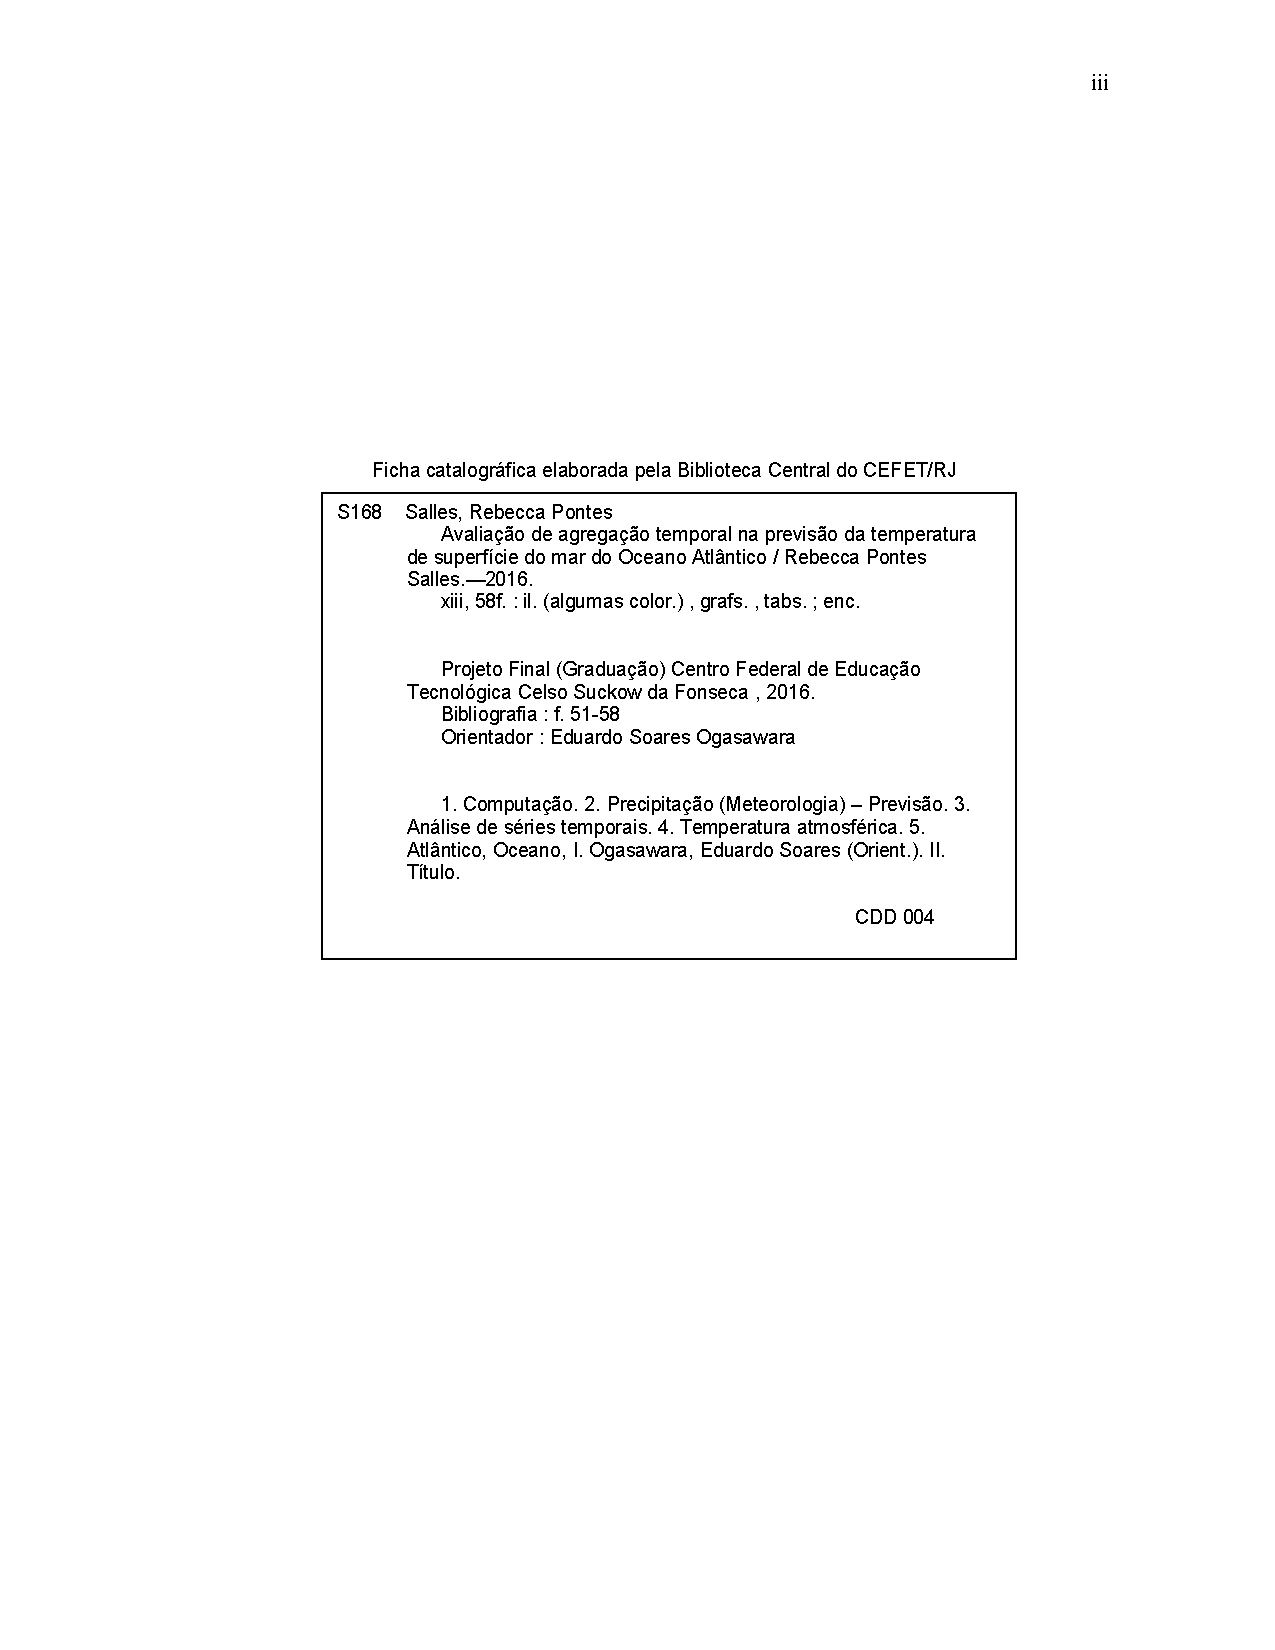
\includepdf{ficha.pdf} % página pdf feita pela biblioteca
	
	\iffalse % COMENTÁRIO
	\center % Center everything on the page
	
	\fbox{%
		\hspace{1cm}
		\parbox{0.6\textwidth}{%
			\footnotesize
			
			Moraes, Luan Marcelo de Aristeu Vilarin Moraes; Moreira, Thiago Della Libera.
			
			\hspace{0.3cm} TOP SECRET / Rebecca Pontes Salles -- 2017. 
			
			\hspace{0.3cm} \pageref{lastpretextualpage},   \pageref{lastpage}f; enc.
			\singlespacing
			\hspace{0.3cm} Projeto Final (Graduação), Centro Federal de Educação Tecnológica Celso Suckow da Fonseca, 2016. 
			
			\hspace{0.3cm} Bibliografia: f, \pageref{bibpage}--\pageref{bibfinalpage}
			
			\doublespacing
			
			\hspace{0.3cm} \textit{1. Modelos de previsão 2. Séries temporais 3. Agregação temporal 4. Temperatura da superfície do mar 5. Oceano Atlântico I. Título}
		}%
	}
	\fi % FIM DO COMENTÁRIO
	
	\pagebreak
	
	%----------------------------------------------------------------------------------------
	%	Dedicatória
	%----------------------------------------------------------------------------------------
	
	{\fontsize{16pt}{\baselineskip}\selectfont \textbf{DEDICATÓRIA}}
	%\thispagestyle{empty}
	\vspace*{15em}%
	\begin{flushright}
		\begin{minipage}{0.5\textwidth}
			\raggedleft \normalsize A Deus e Google, à minha família amada que me ajudaram, apoiaram e guiaram ao longo de toda a minha vida.
		\end{minipage}\\[1.5cm]
	\end{flushright}
	
	\pagebreak
	
	%----------------------------------------------------------------------------------------
	%	Agradecimentos
	%----------------------------------------------------------------------------------------
	
	{\fontsize{16pt}{\baselineskip}\selectfont \textbf{AGRADECIMENTOS}}
	%\thispagestyle{empty}
	\vspace*{10em}%
	\begin{flushright}
		\begin{minipage}{0.5\textwidth}
			\normalsize
			Agradece-se ao \acr{CNPq} pelo financiamento parcial desta pesquisa.\\
			\\
			Agradece-se também as contribuições de ... que deu início a pesquisas sobre o tema abordado.
		\end{minipage}\\[1.5cm]
	\end{flushright}
	
	\pagebreak
	
	%----------------------------------------------------------------------------------------
	%	Resumo
	%----------------------------------------------------------------------------------------
	
	\begin{center}
		{\fontsize{16pt}{\baselineskip}\selectfont \textbf{RESUMO}}\\[2em]
	\end{center}
	
	\justifying 
	\noindent
	O crescente aumento de congestionamentos no tráfego rodoviário demanda pesquisas relacionadas a mobilidade urbana. Essas pesquisas modelam o problema do tráfego como de trajetória, a partir da análise individualizada de objetos móveis que continuamente transmitem sua geolocalização. Um exemplo disso são os ônibus do Rio de Janeiro. Tais veículos funcionam como sensores de trajetória e produzem grande quantidade de dados. Algumas questões, no entanto, continuam em aberto, como características do transporte público em horários de pico e comportamentos sistêmicos presentes nas diferentes regiões que interfiram na mobilidade da cidade. A agregação espaço-temporal dos dados das trajetórias dos modais urbanos oferece uma visão sumarizada dos dados com potencial para identificação de padrões sistêmicos. Este trabalho visa a aplicar técnicas de identificação de motifs sobre esses dados agregados. Espera-se encontrar padrões que expliquem as diferentes formações e propagações de atrasos, bem como outros fenômenos escondidos sob esse grande volume de dados.
	\\[3em]
	
	\normalsize\noindent
	\textbf{Palavras-chave}: modelos de previsão; séries temporais; agregação temporal; temperatura da superfície do mar; Oceano Atlântico
	
	\pagebreak
	
	%----------------------------------------------------------------------------------------
	%	Abstract
	%----------------------------------------------------------------------------------------
	
	\begin{center}
		{\fontsize{16pt}{\baselineskip}\selectfont \textbf{ABSTRACT}}\\[2em]
	\end{center}
	
	\justifying
	\noindent
	Extreme environmental events such as droughts affect millions of people all around the world. Although it is not possible to prevent this type of event, its prediction under different time horizons enables the mitigation of eventual damages caused by its occurrence. An important variable for identifying occurrences of droughts is the \acr{SST}. In the Tropical Atlantic Ocean, \acr{SST} data are collected and provided by the Prediction and Research Moored Array in the Tropical Atlantic (\acr{PIRATA}) Project, which is an observation network composed of sensor buoys arranged in this region. Sensors of this type, and more generally Internet of Things (\acr{IoT}) sensors, commonly lead to data losses that influence the quality of data sets collected for adjusting prediction models. In this paper, we explore the influence of temporal aggregation in predicting step-ahead \acr{SST} considering different prediction horizons and different sizes for training data sets. We have conducted several experiments using data collected by \acr{PIRATA} Project. Our results point out scenarios for training data sets and prediction horizons indicating whether or not temporal aggregated \acr{SST} time series may be beneficial for prediction.
	\\[3em]
	
	\normalsize\noindent
	\textbf{Keywords}: prediction models; time series; temporal aggregation; sea surface temperature; Atlantic Ocean
	
	
	\pagebreak
	
	%----------------------------------------------------------------------------------------
	%	TABLE OF CONTENTS
	%----------------------------------------------------------------------------------------
	
	\renewcommand{\cftdot}{}
	\tableofcontents % Include a table of contents 
	
	\pagebreak
	
	%----------------------------------------------------------------------------------------
	%	TABLE OF FIGURES
	%----------------------------------------------------------------------------------------
	
	\listoffigures
	
	\pagebreak
	
	%----------------------------------------------------------------------------------------
	%	TABLE OF TABLES
	%----------------------------------------------------------------------------------------
	
	\listoftables
		
	\pagebreak
	
	%----------------------------------------------------------------------------------------
	%	Lista de Abreviações
	%----------------------------------------------------------------------------------------
	
	\printterms[database=acronym,columns=1,prelocation=hfill,style=align]
	
	\label{lastpretextualpage}
	\pagebreak
	
	
	\pagenumbering{arabic}
	\justifying
	
\chapter{Introdução}
\label{sec:introducao}
A cada nova atualização do código-fonte, há chances de que mudanças ocorram na implementação arquitetural do software. Tais mudanças podem gerar discrepâncias à arquitetura previamente definida\citep{Perry:1992:FSS:141874.141884}. Este fenômeno se chama erosão arquitetural e pode trazer sérios riscos ao projeto quando não resolvida antes que possa ser muito custoso para tratar.\citep{Foote99bigball}.

Com o intuito de contornar problemas deste tipo, existem ferramentas que fazem checagem contínua da arquitetura desejada contra a implementada no código-fonte baseando-se em regras programadas em conformidade com a necessidade arquitetural das partes interessadas. A cada alteração no código-fonte, a ferramenta verifica a existência de uma violação arquitetural. Imediatamente, a ferramenta de checagem contínua mostra onde a violação ocorreu ao desenvolvedor. 
////CHECAR REFERENCIA AQUI EMBAIXO
Para grandes projetos, onde o número de violações pode atingir uma quantidade difícil de ser detectada e corrigida, a verificação contínua ajuda a remover inconformidades do código, assim que ela ocorre\citep{goldstein_automatic_2015}.

A ferramenta de checagem contínua de código-fonte que este trabalho abordará será o \textit{SonarQube} \citet{sonar_qube}. Esta ferramenta oferece diversos recursos como, a correção de \textit{bugs}, o auxílio à manutenção de boas práticas de programação. Entretanto, a ferramenta não atende com eficiência quando há a necessidade de criar regras customizadas de arquitetura. Regras que verificam violações de requisitos não-funcionais, são difíceis de serem implementadas. A criação dessas regras requer que o desenvolvedor crie diversos arquivos e implemente com certo esforço de desenvolvimento. 

Neste trabalho, o objetivo principal será estudar formas de criar regras de forma mais prática dentro da ferramenta, isto é com uma linguagem mais expressiva e que possa reduzir o esforço de desenvolvimento. Ao criar uma regra, é desejável que a preocupação principal do desenvolvedor ou arquiteto seja a criação das regras e não as barreiras de implementação das regras da ferramenta. O \textit{SonarQube} é uma ferramenta multi-linguagem. Com o intuito de reduzir o escopo do trabalho, o objetivo foi aprimorar a criação das regras na ferramenta em linguagem Java. Isso foi feito, criando uma linguagem mais simples e expressiva como uma camada superior a linguagem Java. Vale ressaltar, que a escrita de regras na ferramenta para checagem do código-fonte escrito em Java é feita na linguagem Java.

/////MELHORAR PARAGRAFO ABAIXO
Incluindo esta introdução (i), este trabalho foi dividido em quatro outras seções: A fundamentação teórica (ii) reúne trabalhos que, analogamente, pavimentam a estrada na qual este trabalho percorre. O desenvolvimento(iii) descreve a abordagem posta em prática para solucionar o problema apontado e as (iv) conclusões parciais apresentam o que foi aprendido e os planos para a conclusão total do trabalho.


\chapter{Preliminares}
\label{sec:background}
Séries espaço-temporais são definidas como sequência de observações que contêm dados sobre o local e momento em que coleta foi feita \citep{cressie2015statistics}(explicar framework). As séries espaço-temporais podem ser caracterizadas como observações de objetos móveis ou objetos permanentes(explicar potencial de um framework). Os objetos que tem dados de sua localização variantes com o tempo são classificados como móveis. A sequência de observações sobre objetos móveis é classificada como trajetória. A trajetória é o modelo de dados mais aplicado a problemas relacionados ao tráfego \citep{chen2015survey}. Entretanto, estudos que se relacionam mais diretamente com o tema deste trabalho são aqueles em que se agrega informações do objeto \citep{tao2004spatio}, gerando séries espaço-temporais associados a objetos permanentes(explicar que vamos focar mais em trabalho de avaliação de direção senão o escopo vai ficar imenso).

A agregação de dados de objetos móveis pode ser feita de diferentes formas. Os tipos básicos de agregações existentes são Espacial (\emph{S}), Temporal (\emph{T}) e Atributiva ou categórica (\emph{A}). Outros tipos de agregação podem ser feitos a partir da combinação dos tipos básicos, como \emph{$S \times T$}, \emph{$S \times T \times A$} e \emph{$S \times S \times T \times T$} \citep{chen2015survey}. Neste trabalho, a agregação aplicada é a Espaço-Temporal (\emph{$S \times T$}), em que o resultado esperado é composto por séries temporais (T) associadas a pontos geográficos permanentes (S). Tais agregações podem ser interpretadas como sensores virtuais correspondente a região agregada.  

As séries temporais apresentam subsequências que se repetem com frequência. Alguns dos padrões que se repetem não são conhecidos, configurando \emph{motifs} \citep{esling2012time}. A identificação de \emph{motifs} podem ser feita sobre séries temporais univariadas ou multivariadas. Neste trabalho, as séries espaço-temporais obtidas após a agregação \emph{$S \times T$} são multivariadas \citep{wang2016effective} \citep{vahdatpour2009toward}. 


\chapter{Trabalhos Relacionados}
\label{sec:trabalhos_relacionados}
Diversos trabalhos propõem-se a coletar e interpretar informações de modo a identificar padrões que respondam questionamentos acerca da qualidade do serviço de transporte multimodal em várias localidades do planeta. Inúmeros fatores podem vir a influenciar o conforto da viagem e o grau de satisfação do passageiro para com a experiência entregue pela companhia de transporte. 

Algumas características podem porém gerar danos à segurança dos passageiros. \citep{world2015global} aponta a relação entre a condição da malha viária e o índice de acidentes fatais no trânsito. \citep{euPolicyDep} afirma que o comportamento do motorista é, juntamente com a qualidade da infraestrutura disponível, o maior contribuidor para que acidentes aconteçam. Logo, é possível achar uma justificativa plausível para que tantos trabalhos tentem identificar padrões nas viagens afim de tentar mitigar algumas das situações apontadas como possíveis causas de acidentes.

Utilizando-se de estratégias menos complexas ou mais robustas, inúmeros são os trabalhos dedicados ao levantamento e processamento de informações para entender e melhorar a infraestrutura das estradas ou o comportamento do motorista no trânsito. \citep{gawad2016dynamic} propõem uma abordagem de detecção de anomalias na pista utilizando aprendizado de máquina para calcular o limite entre um balanço natural do automóvel e um buraco no asfalto. Seu trabalho é dividido entre a aplicação em um telefone móvel, utilizada para perceber anomalias e apresentar um mapa com as marcações de outros eventos levantados anteriormente por mais usuários. E, um servidor que utiliza aprendizado por reforço para inserir ou remover anomalias no banco de dados. 

\citep{HANAOKA2014274} estuda a aplicabilidade de interpretar dados sobre o trajeto diário de estudantes da Universidade de Ritsumeikan em Kyoto, Japão. Em seu trabalho, os autores estimam as rotas dos estudantes interpolando dados de serviços multimodais de transporte que representam a origem e o destino dos estudantes em horários restritos do dia. Utilizando esta abordagem tenta-se prever o deslocamento de estudantes e a área de maior concentração dos mesmos na respectiva fatia temporal diária. Podendo assim o trafego ao redor da universidade e a oferta de transporte até a mesma serem melhor estruturados.

Em \citep{kim2009passenger} apresenta-se uma modelagem a partir de uma entrevista em forma de questionário que visa predizer o comportamento de passageiros baseado na probabilidade de escolha entre o primeiro ônibus a chegar à parada e o segundo. Tendo como características determinante o conforto da viagem baseado na disponibilidade de assentos, lotação do veículo e o tempo de duração do trajeto.

Já \citep{raymond2016} debruça-se sobre a questão da difícil interpretação de séries-temporais advindas do sistema GPS, já que as mesmas podem vir a apresentar \textit{outliers} cuja origem é a interferência que o sinal de geolocalização pode vir a receber. Para evitar tratar tal desafio é utilizado uma técnica de correspondência por mapas (\textit{map-matching}) e \textit{bag of words}, esta última sendo uma técnica de classificação de imagem. A correspondência por mapas transforma uma sequência de pontos do GPS em uma de ruas, diminuindo a granularidade do problema. Para testar tal abordagem é utilizado a base de dados de posições dos ônibus da cidade do Rio de Janeiro. 

\cite{SINGH201756}


\begin{table}[!ht]
	\centering
	\caption{Comparação dos trabalhos relacionados}
	\begin{tabular}{ L{6cm} C{1.5cm} C{1.5cm} C{1.5cm} C{1.5cm} }
		\hline\noalign{\smallskip}
		Trabalho & AETR  & AETP & IMS  & IMT \\
		\hline\noalign{\smallskip}
		%\hline\noalign{\smallskip}
		\citet{ferreira2013visual} & X &  &  & \\
		\citet{andrienko2008spatio} & X &  &  & \\
		\citet{adrienko2011spatial} &  & X &  & \\
		\citet{cassisi2013motif} &  &  & X & \\
		\citet{jiang2008finding} &  &  & X & \\
		\citet{chi2012face} &  &  & X & \\
		\citet{schneider2013unravelling} &  &  &  & X \\
		\hline\noalign{\smallskip}
	\end{tabular}
	\label{tbl:sumario}
\end{table}

A tabela \ref{tbl:sumario} apresenta os trabalhos relacionados e as técnicas aplicadas. Áreas mais exploradas são a identificação de \emph{motifs} em séries temporais e a agregação espaço-temporal baseada em região. Não foram observados trabalhos associados a identificação de \emph{motifs} em séries espaço-temporais associadas a objetos permanentes. Observa-se, portanto, uma lacuna para estudo com amplo potencial de exploração.

\chapter{Proposta} 
\label{sec:proposta}
Este trabalho tem como objetivo facilitar o desenvolvimento de aplicações de coletas de dados gerais através dos sensores de um smartphone convencional ao avaliar a qualidade de direção mas não restringido apenas a esse proposito. Como citado na seção de trabalhos relacionados, a grande maioria dos trabalhos partia de um ponto inicial onde não havia nenhuma ferramenta que auxiliasse ou facilitasse a execução da pesquisa. Todos os trabalhos coletavam dados crus e trabalhavam em cima dos mesmo com, em certos casos filtros e çalculos para normalizarem os dados e assim, poder fazer uma análise dos mesmos. Mesmo tendo esse conceito em mente, a proposta de um framwork é muito mais ampla que atacar somente esse tipo de usuário. Existem possibilidades de que este framework seja utiliado no mercado por sua fácil customização e sua modularização.

A criação de um framework tem o objetivo de generalizar e facilitar a execução de qualquer tarefa sem que a mesma seja retrabalhada, seja em metodologia ou desenvolvimento, com certo grau de customização.(um objetivo). Estão sendo considerados trabalhos nos quais o objetivo é coetar e interpretar dados dos sensores do celular como acelerometro, GPS, sensor de gravidade, giroscópio(nem sei se existe, inventei). Como a extensão do uso de um framework é muito ampla, o escopo será reduzido para atender necessidades voltadas ao processamento e avaliação da qualidade e perfil de direção de motoristas em geral.Ainda assim podemos extrai um grande quantidade de possibilidades em relação a que tipo de motorista será o alvo do trabalho. Portanto, ao final deste trabalho será apresentado uma aplicação exemplo que irá coletar dados sobre o delsocamento dos alunos do CEFET e avaliar se a qualidade dos meios de transporte utilizados é satisfatória. 

esta avaliação é feita desta forma (elaborar isso conforme o trabalho é desenvolvido mas aqui seria interessante falar do app exemplo no qual o framework irá atuar)

Uma vez que as séries espaço-temporais sejam produzidas, aplica-se a identificação de \emph{motifs} sobre essas séries. Em função das propriedades destes dados, pretende-se desenvolver um algoritmo, inspirado em \emph{random projection} \citep{li2009probabilistic}, que introduza restrições espaço-temporais na identificação destes padrões. Estas restrições espaço-temporais visam observar padrões que se propagam ao longo de uma vizinhança(conclusão da aplicação de toda nossa metodologia). Deste modo, espera-se que sejam emanados padrões capazes de responder as questões de pesquisa previamente mencionadas(o que se espera).  

\chapter{Estado Atual do Trabalho}
\label{sec:estado_atual}

Seguindo o processo de implementação descrito na Seção \ref{sec:proposta}, inicialmente foram definidas as estações (1:Estações) que funcionam como pontos permanentes à agregação espaço-temporal. O primeiro passo é converter os dados geodésicos em um plano cartesiano. Para tanto, foi definido um ponto inicial $P\textsubscript{0}(lat, long)$ referente a menor latitude e longitude do espaço amostral. Em seguida, os pontos de ônibus foram convertidos em pares ordenados, de modo que um ponto de ônibus $P\textsubscript{1}(lat,long)$ seja convertido em $P(x,y)$ tal que $x$ e $y$ são a distância \emph{Harversine} entre $P\textsubscript{2}(lat\textsubscript{P\textsubscript{0}},long\textsubscript{P\textsubscript{1}})$ e $P\textsubscript{0}$ e a distância \emph{Harversine} entre $P\textsubscript{3}(lat\textsubscript{P\textsubscript{1}},long\textsubscript{P\textsubscript{0}})$, respectivamente. Os valores de $x$ e $y$ estão representados na Figura \ref{fig:conversao}.

\begin{figure}[!ht]
	\centering
	\begin{minipage}[t]{0.49\textwidth}
		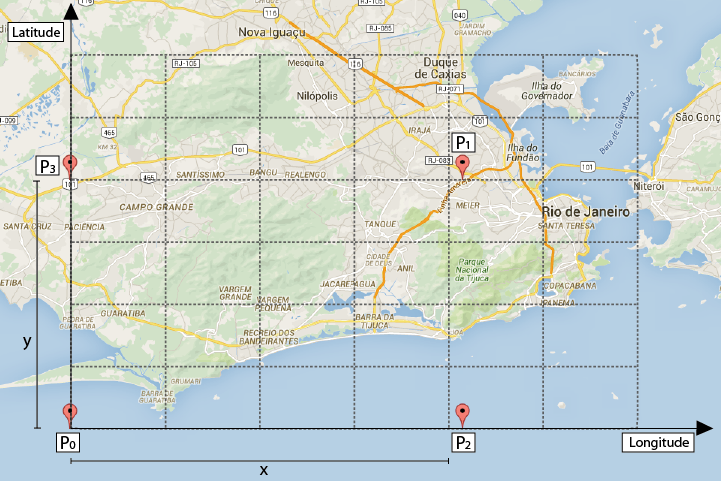
\includegraphics[width=\textwidth]{conversao.png}
		\caption
		{
			Conversão dos dados de localização dos pontos de ônibus.
		}
		\label{fig:conversao}
	\end{minipage}
	\hfill
	\begin{minipage}[t]{0.47\textwidth}
		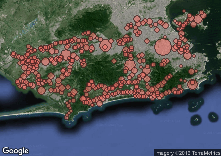
\includegraphics[width=\textwidth]{stations-v3.png}
		\caption
		{
			Estações obtidas aplicando o algoritmo de agrupamento DBSCAN sobre os pontos de ônibus do Rio de Janeiro.
		}
		\label{fig:stacoes}
	\end{minipage}	
\end{figure}

Os pares ordenados obtidos com o processo de conversão dos dados de localização dos pontos de ônibus foram agrupados por DBSCAN, considerando \emph{eps} de 300 metros e o mínimo de um ponto. A partir dos 7020 pontos de ônibus obtidos pelo Portal de Dados Abertos do Rio de Janeiro, foram geradas 307 estações. Na Figura \ref{fig:stacoes}, os marcadores vermelhos indicam as estações obtidas após o agrupamento dos pontos de ônibus. O tamanho do marcador é proporcional a quantidade de pontos que foram agrupados.

As observações de GPS sobre os ônibus da cidade do Rio de Janeiro devem ser associadas às estações, de modo que cada observação seja associada a estação mais próxima. Em seguida, os dados foram agregados às estações, considerando um $\Delta t$ de 1 minuto. No processo de agregação foram obtidos dados referentes a contagem de linhas e de ônibus, velocidade média de ônibus associados a estação e listagem das linhas e dos ônibus associados a estação no momento. Inicialmente, o processo foi executado sobre dados do dia 26 de junho de 2015. Das mais de 4 milhões de observações individuais de ônibus, foram geradas 278.307 observações agregadas.

Além da agregação considerando o $\Delta t = 1 minuto$ , serão realizadas agregações espaço-temporais considerando o $\Delta t = 4 minutos$ e $\Delta t = 8 minutos$. Após o processo de agregação (2:Agr.Temp.), teremos como resultado séries espaço-temporais associadas a pontos permanentes. Com as séries espaço-temporais definidas, o desenvolvimento de algoritmos para identificação de \emph{motifs} (3:Id.Motifs) será realizada. A conclusão prevista para os algoritmos \textit{motifs} é janeiro de 2017, abrindo espaço para experimentação (4:Aval.Exp.) e análise dos resultados obtidos (5:Ana.Result.). 

As pesquisas e a produção textual estão sendo realizada em paralelo às demais etapas. A fundamentação teórica (6:Fund.Teo.) se encontra em fase de desenvolvimento e tem conclusão prevista para setembro de 2016. A solução proposta (7:Metodologia) neste trabalho será descrita de forma mais precisa e detalhada até janeiro de 2017. O experimento e seus resultados serão explorados após a etapa de experimentação, levando em conta a produção de artigo (8:Artigo) associado. 

A defesa da dissertação (9:Defesa) está prevista para setembro de 2017. O cronograma, indicado na tabela \ref{tbl:cronograma}, prevê as etapas abordadas neste trabalho. A tabela indica os meses de previsão de conclusão de cada uma das etapas.

\begin{table}[!ht]
	\centering
	\caption{Cronograma de desenvolvimento da dissertação}
	\begin{tabular}{ L{3cm} C{1cm} C{1cm} C{1cm} C{1cm} C{1cm} C{1cm} C{1cm} C{1cm} C{1cm} }
		\hline\noalign{\smallskip}
		Atividade & jun-jul  & ago-set & out-nov & dez-jan & fev-mar & abr-mai & jun-jul & ago-set \\
		\hline\noalign{\smallskip}
		1:Estações & X & & & & & & & \\
		2:Agr.Temp. & X & X & & & & & & \\
		3:Id.Motifs & & & X & X & & & & \\
		4:Aval.Exp. & & & & X & & & & \\
		5:Ana.Result. & & & & & X & X & & \\
		6:Fund.Teo.& X & X & & & & & & \\
		7:Metodologia & & X & X & X & & & & \\
		8:Artigo & & & & & X & X & X & \\
		9:Defesa & & & & & & & & X \\
		\hline\noalign{\smallskip}
	\end{tabular}
	\label{tbl:cronograma}
\end{table}

\label{bibpage}
\addcontentsline{toc}{section}{Referências Bibliográficas}
\bibliography{references}
\bibliographystyle{plain}
\label{bibfinalpage}


\label{lastpage}\end{document}
